\chapter{Marco te\'orico}\label{capit:cap2}
\vspace{-2.0325ex}%
\noindent
\rule{\textwidth}{0.5pt}
\vspace{-5.5ex}% 
\newcommand{\pushline}{\Indp}% Indent puede ir o no :p

En este capítulo se definen una serie de conceptos importantes del área de procesamiento de imágenes y reconocimiento de patrones, estas definiciones son importantes para la comprensión del tema.



\section{Gestos}\label{sec:2Gestos}
Los gestos \citep{Mitra2007} son movimientos del cuerpo expresivos y significativos que involucran dedos, manos, brazos, cabeza, cara o cuerpo con la intención de transmitir información relevante o interactuar con el ambiente. De acuerdo con la literatura \citep{Mitra2007} los gestos con las manos se clasifican en estáticos y dinámicos, los primeros están definidos como la posición y orientación de la mano en el espacio manteniendo esta pose durante cierto tiempo, por ejemplo para hacer una se\~nal de aventón, a diferencia de los gestos dinámicos donde hay movimiento de la pose, un ejemplo  es cuando mueves la mano en se\~nal de adiós. De aquí en adelante entiéndase el término gestos con las manos, como gestos.  



\section{Reconocimiento de gestos con la manos}\label{sec:2ReconocimientoGestos}  

El reconocimiento de gestos se divide en tres fases \citep{Rautaray2012}, detección o segmentación; extracción de características seguimiento; dependiendo si los gestos son dinámicos, por último la etapa final el reconocimiento del gesto.  
Este se clasifican en dos modelos, basados en la visión y en contacto, esta clasificación depende de la manera en que son capturados los datos, es decir la forma en que se obtiene el gesto, para posteriormente poderlo reconocer. 

Los primeros acercamientos para llevar acabo el reconocimiento de gestos fue usando modelos de contacto \citep{Rautaray2012} y \citep{Nayakwadi2014}, como su nombre lo dice utilizan dispositivos que est\'an en contacto f\'isico con la mano del usuario, esto para capturar el gesto a reconocer, por ejemplo existen guantes de datos, marcadores de colores, acelerómetros y pantallas multi-touch, aunque estos no son tan aceptados pues entorpecen la naturalidad entre la interacción del humano y la computadora. Los modelos basados en la visión surgieron como respuesta a esta desventaja, estos utilizan cámaras para extraer la información necesaria para realizar el reconocimiento, los dispositivos van desde c\'amaras web hasta algunas más sofisticadas por ejemplo c\'amaras de profundidad.  

Los métodos basados en la visión se pueden representar por dos modelos \citep{Rautaray2012}, los basados en 3D, da una descripción espacial en 3D de la mano, y los basados en apariencia, como su nombre lo dice se basan en la apariencia de la mano. Los modelos basados en apariencia se dividen en dos categorías, los estáticos (modelo de silueta, de contorno deformables) y de movimiento (de color y movimiento).

\subsection{Etapas del reconocimiento}\label{subsec:EtapasReconocimiento} 
Enseguida se describen las etapas del reconocimiento de gestos \ref{fig:HGR}, con los métodos para llevar cada una de estas.  

\begin{figure}[h!]
\begin{center}
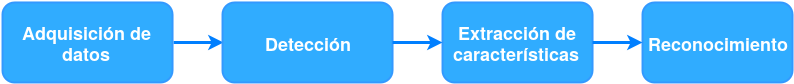
\includegraphics[scale=.8]{./Figures/HGR.png}
\end{center}
\caption{Procedimiento del algoritmo de detección}
\label{fig:HGR}
\end{figure}

\subsubsection{Detección}\label{sssec:EtapaDeteccion}

En esta etapa se detecta y segmenta la información relevante de la imagen (la mano), con la del fondo, existen distintos métodos para obtener dichas características como la de color de la piel, forma, movimiento, entre otras que generalmente son combinaciones de alguna de estas, para obtener un mejor resultado. Enseguida se describe brevemente cada una de estas.  
\begin{itemize}
\item Color de la piel: Se basa principalmente en escoger un espacio del color, es una organización de colores especifica; como; RGB (rojo, verde, azul), RG (rojo, green), YCrCb (brillo, la diferencia entre el brillo y el rojo, la diferencia entre el brillo y el azul), etc. La desventaja es que si es color de la piel es similar al fondo, la segmentación no es buena, la forma de corregir esta segmentación es suponiendo que el fondo no se mueve con respecto a la cámara.
\item Forma: Extrae el contorno de las imágenes, si se realiza correctamente se obtiene el contorno de la mano. Aunque si se toman las yemas de los dedos como características, estas pueden ser ocluidas por el resto de la mano, una posible solución es usar más de una cámara.  
\item Valor de p\'ixeles: Usar imágenes en tonos de gris para detectar la mano en base a la apariencia y textura, esto se logra entrenando un clasificador con un conjunto de imágenes.
	\item Modelo 3D: Depende de cual modelo se utilice, son las características de la mano requeridas. 
	\item Movimiento: Generalmente esta se usa con otras formas de detección ya que para utilizarse por sí sola hay que asumir que el único objeto con movimiento es la mano.
\end{itemize}

\subsubsection{Seguimiento}\label{sssec:EtapaSeguimiento}

Consiste en localizar la mano en cada cuadro (imagen). Se lleva acabo usando los métodos de detección si estos son lo suficientemente rápidos para detectar la mano cuadro por cuadro. Se explica brevemente los métodos para llevar a cabo el seguimiento. 
\begin{itemize}
	\item Basado en plantillas: Este se divide en dos categorías (Características basadas en su correlación y basadas en contorno), que son similares a los métodos de detección, aunque supone que las imágenes son adquiridas con la frecuencia suficiente para llevar acabo el seguimiento. Características basadas en su correlación, sigue las características a través de cada cuadro, se asume que las características aparecen en mismo vecindario. Basadas en contorno, se basa en contornos deformables, consiste en colocar el contorno cerca de la región de interés e ir deformando este hasta encontrar la mano. 
	\item Estimación óptima: Consiste en usar filtros Kalman, un conjunto de ecuaciones matemáticas que proporciona una forma  computacionalmente eficiente y recursiva de estimar el estado de un proceso, de una manera que minimiza la media de un error cuadrático, el filtro soporta estimaciones del pasado, presente y futuros estados, y puede hacerlo incluso cuando la naturaleza precisa del modelo del sistema es desconocida;  para hacer la detección de características en la trayectoria. 
	\item Filtrado de partículas: Un método de estimación del estado de un sistema que cambia a lo largo del tiempo, este se compone de un conjunto de partículas (muestras) con pesos asignados, las partículas son estados posibles del proceso. Es utilizado cuando no se distingue bien la mano en la imagen. Por medio de partículas localiza la mano la desventaja es que se requieren demasiadas partículas, y el seguimiento se vuelve imposible. 
	\item Camshift: Busca el objetivo, en este caso la mano, encuentra el patrón de distribución mas similar en una secuencia de imágenes, la distribución puede basada en el color. 
\end{itemize}

\subsubsection{Reconocimiento}\label{sssec:EtapaReconocimiento}

Es la clasificación del gesto, la etapa final del reconocimiento, la clasificación se puede hacer dependiendo del gesto. Para gestos estáticos basta con usar algún clasificador o empatar el gesto con una plantilla. En los dinámicos se requiere otro tipo de algoritmos de aprendizaje de máquina. A continuación se encuentran los principales métodos para llevar acabo el reconocimiento del gestos. 
\begin{itemize}
	\item K-medias: Consiste en determinar los $k$ puntos llamados centros para minimizar el error de agrupamiento, que es la suma de las distancias de todo los puntos al centro de cada grupo. El algoritmo empieza localizando aleatoriamente $k$ grupos en el espacio espectral. Cada p\'ixel en la imagen de entrada es entonces asignadas al centro del grupo mas cercano  
	\item {K-vecinos cercanos} (KNN, por sus siglas en ingl\'es): 
	Este es un método para clasificar objetos basado en las muestras de entrenamiento en el espacio de características. 
	\item Desplazamiento de medias: Es un método iterativo que encuentra el máximo en una función de densidad dada una muestra estadística de los datos.
	\item Máquinas de soporte vectorial (SVM, por sus siglas en ingl\'es). Consiste en un mapeo no lineal de los datos de entrada a un espacio de dimensi\'on m\'as grande, donde los datos pueden ser separados de forma lineal.  
	\item Modelo oculto de Markov (HMM, por sus siglas en ingl\'es) es definido como un conjunto de estados donde un estado es el estado inicial, un conjunto de símbolos de salida y un conjunto de estados de transición. En el reconocimiento de gestos se puede caracterizar a    los estados como un conjunto de las posiciones de la mano; las  transiciones de los estados como la probabilidad de transición de cierta posición de la mano a otra; el símbolo de salida como una postura especifica y la secuencia de los símbolos de salida como  el gesto de la mano.   
	\item Redes neuronales con retraso: Son una clase de redes neuronales artificiales que se enfocan en datos continuos, haciendo que el sistema sea adaptable para redes en linea y les da ventajas sobre aplicaciones en tiempo real. 
\end{itemize}  



\section{Imagen}\label{ImagenDef} 

Una imagen se puede definir como una función bidimensional, $S(x,y)$ donde $x$, $y$ representan las coordenadas en el plano y el valor de la función es la intensidad o nivel de gris en el punto $(x,y)$. 
Si el valor de la función y los puntos de la imagen son finitos, esta es una imagen digital, la cual se puede representar en una matriz donde cada valor o pixel es el nivel de gris de la imagen, y los indices de esta indican la posición, \citep{Gonzalez2002}. 



\section{Oclusión}\label{OclusionDef} 

Se puede definir una oclusión como discontinuidades del movimiento y profundidad que se es percibida por un observador que se encuentra en movimiento en un ambiente estático.\\
Los puntos de oclusión en una imagen o cuadro son pixeles que aparecen o desaparecen en dos cuadros consecutivos, estos son llamados puntos de oclusión o punto de no oclusión, \citep{Silva2001}.  

Existen tres tipos distintos de oclusiones la cuales depende de la forma en que es causada. Estas son: oclusión por el mismo objeto, entre objetos y por el fondo. La oclusión por el mismo objeto se presenta cuando parte del objeto ocluye a otra. La oclusión entre objetos es cuando dos objetos que se siguen se ocluyen entre ellos mismos. La oclusión por el fondo es cuando parte del fondo ocluye al objeto que se sigue, \citep{YilmazA.JavedO.andShah2006}


\newpage
%%=====================================================
